% !TEX encoding = UTF-8
% !TEX TS-program = pdflatex
% !TEX root = ../tesi.tex
% !TEX spellcheck = it-IT

%*********************************************************
\chapter{SLA Management}
\begin{flushright}
\textit{a cura di \large{Marco Casagrande}}
\end{flushright}
\label{cap:slamanagement}
%**********************************************************

\section{Panoramica generale}

\subsection{Consegna}

Pianificazione ed organizzazione del processo di SLA Management; secondo quanto indicato nel Capitolato Tecnico dell'Azienda Ospedaliera Gaetano Pini, sezione 5.1.4.5 - Misurazione dei livelli di Servizio (SLA Management):
\\

\textit{"Il Service Level Agreement (SLA) è un accordo tra un utente e un fornitore di un servizio che definisce la natura del servizio fornito e stabilisce un insieme di parametri da utilizzare per misurare il livello del servizio erogato. L’accordo può essere molto dettagliato ed includere la definizione di ruoli, delle responsabilità e dei termini da cui far decorrere le penali. 
\\ \\
La Gestione dei Livelli di Servizio (SLA Management) è il processo che riguarda il governo dei Livelli di Servizio richiesti nel presente capitolato e/o proposti nell’Offerta Tecnica e riportati nel Contratto. Il processo focalizza gli aspetti peculiari della preparazione (e/o rinnovo), registrazione, e controllo dei Livelli di Servizio contrattuali.
\\ \\
L’Istituto chiede ai concorrenti di fornire i servizi di gestione in questa ottica di SLA. Pertanto l’offerente dovrà organizzare il servizio con l’obiettivo di poter documentarne la rispondenza a dei parametri (livelli) precedentemente definiti, in modo condiviso e concorde, con l’Istituto. L’offerente dovrà descrivere le attività di SLA management di cui si farà carico durante la gestione, indicando anche gli strumenti che intende utilizzare per registrare e documentare il livelli di servizio.
\\ \\
L’offerente deve quindi proporre un sistema informativo dedicato alla gestione degli SLA, “lo SLA Manager”, che ha quindi come obiettivo finale l’esposizione dello stato effettivo del servizio erogato. Tutto ciò, ponendo in relazione i livelli di servizio erogati con le norme che regolano contrattualmente l’erogazione del servizio in generale, attraverso indicatori oggettivamente misurabili, esplicitamente richiesti dall’Istituto e/o proposti dall’offerente sulla base del proprio know how.
\\ \\
L’Istituto richiede che, tramite opportune funzionalità, si possa verificare in qualsiasi momento, in modo autonomo e disgiunto (da parte dell’Istituto o dell’offerente), lo stato del servizio e di conseguenza il rispetto dei termini contrattuali."}

\subsection{Definizione degli obiettivi}

I punti chiave del processo di SLA Management, estrapolati dalle richieste presenti nel capitolato sono:

\begin{itemize}
	\item la definizione delle attività di preparazione, rinnovo, registrazione e controllo degli SLAs;
    \item la definizione degli strumenti necessari e di un sistema informativo a supporto del processo.
\end{itemize}

Il processo di Service Level Management, definito nel framework ITIL, è estremamente affine a quanto richiesto per il processo di SLA Management. Lo sfrutteremo dunque come base di partenza.

\begin{figure}[H]
\centering
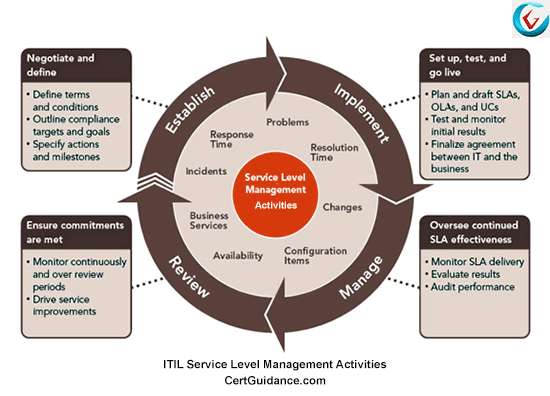
\includegraphics[width=30em]{immagini/sla/slmdiagram.png}
\caption{Diagramma ITIL del processo di Service Level Management}
\end{figure}

Il processo di Service Level Management si occupa di:

\begin{itemize}
	\item definire ed organizzare un Service Catalogue dei servizi erogati dal fornitore;
	\item progettare i Service Level Requirements per i nuovi servizi;
    \item trasformare gli SRL in Service Level Agreements;
    \item definire gli Operational Level Agreements e gli Underpinning Contracts necessari a garantire gli SLAs concordati;
    \item monitorare le performance di SLAs, OLAs, UCs e produrre report ad intervalli regolari;
    \item condurre indagini e review sulla qualità e sui possibili miglioramenti dei servizi rispetto agli SLAs, secondo i Service Improvement Programs;
    \item gestire i rapporti con i clienti per garantirne la soddisfazione.
\end{itemize}

Il processo di Service Level Management ospita quattro sotto-processi:

\begin{itemize}
	\item Maintenance of the SLM Framework, con lo scopo di progettare e mantenere il Customer Agreement Portfolio e fornire i template dei documenti necessari al processo di SLM;
    \item Identification of Service Requirements, con lo scopo di catturare i desideri dei clienti per dei nuovi servizi o per delle modifiche a quelli preesistenti;
    \item Agreements Sign-Off and Service Activation, con lo scopo di finalizzare le sottoscrizioni ai contratti di SLAs, OLAs, UCs e verificare i Service Acceptance Criteria;
    \item Service Level Monitoring and Reporting, con lo scopo di monitorare le prestazioni dei servizi rispetto a quelle concordate e diffondere i Service Level Reports.
\end{itemize}

Le richieste presentate nel Capitolato Tecnico rispetto al processo di SLA Management trovano corrispondenza nel processo ITIL di Service Level Management. Quest'ultimo pone inoltre obiettivi di qualità ed enfasi sulle relazioni con i clienti, entrambi non espressamente richiesti nel Capitolato Tecnico. Durante l'implementazione del nuovo processo di SLA Management attribuiremo una priorità inferiore a tali aspetti, in quanto ritenuti meno interessanti dal cliente.

\subsection{Fonti}

Vengono qui riportate le fonti cui ho attinto per conoscenze ed ispirazione allo scopo di redigere il capitolo SLA Management:

\begin{itemize}
	\item \href{http://www.netadm.it/admsys_2018/admsys.htm}{Corso di Amministrazione di Sistema 2017/2018}, in particolare le slide delle lezioni;
    \item \href{https://wiki.en.it-processmaps.com/index.php/Main_Page}{IT Process Wiki}, per qualsiasi approfondimento legato ai processi ITIL ma anche alle checklist per i documenti SLA, OLA ed UC;
    \item \href{https://www.teamquest.com/files/6614/2049/9759/itil4.pdf}{TeamQuest}, per la descrizione approfondita sull'implementazione del processo ITIL di Servel Level Management;
    \item \href{https://www.hci-itil.com/ITIL_v3/docs/3792_itil_ebook_1.pdf}{HCI-ITIL}, per la descrizione approfondita sull'implementazione del processo ITIL di Servel Level Management;
    \item \href{https://www.theitsmhub.com.au/wp-content/uploads/2014/12/A-Practical-Approach-to-Implementing-Service-Level-Management.pdf}{Pink Elephant}, per la descrizione approfondita sull'implementazione del processo ITIL di Servel Level Management;
        \item \href{https://www.pinkelephant.com/uploadedFiles/Content/ResourceCenter/PinkPapers/ImplementingServiceLevelManagement.pdf}{Pink Elephant}, per un ulteriore punto di vista sul processo ITIL di Servel Level Management;
    \item \href{https://wiki.scn.sap.com/wiki/display/SAPITSM}{SAP Community Wiki}, in particolare i vari post riguardo all'implementazione di processi ITIL tramite SAP Solution Manager;
    \item \href{https://support.sap.com/en/index.html}{SAP Support Portal}, per l'approfondimento riguardo allo strumento software SAP Solution Manager;
    \item \href{https://help.sap.com/viewer/index}{SAP Help Portal}, per l'approfondimento riguardo allo strumento software SAP Solution Manager;
    \item \href{https://tsd.gmu.edu/policies/SLAs/}{George Mason University}, per un template di SLA;
    \item \href{https://tsd.gmu.edu/policies/olas.cfm}{George Mason University}, per un template di OLA;
    \item \href{https://its.ucsc.edu/itsm/servicemgmt.html#definition}{UC Santa Cruz}, per un template di SLA;
    \item \href{https://its.ucsc.edu/itsm/servicemgmt.html#definition}{UC Santa Cruz}, per un template di OLA;
    \item \href{http://www.axia-consulting.co.uk/html/sla_metrics.html}{Axia-Consulting}, per informazioni sulle metriche degli SLAs;
    \item \href{http://www.slatemplate.com/}{ SLA Template.com}, per un template di SLA;
    \item \href{https://www.certguidance.com/topics/itil-foundation/}{CertGuidance}, per alcuni articoli e l'immagine del diagramma SLM;
    \item \href{https://www.uptrends.com/}{Uptrends}, per l'approfondimento riguardo allo strumento software Uptrends;
    \item \href{https://www.happyfox.com/}{happyfox}, come possibile strumento informatico;
    \item \href{https://www.webhelpdesk.com/help-desk-software/sla-management-monitoring-reports}{web help desk}, come possibile strumento informatico;
    \item \href{https://www.dotcom-monitor.com/web-performance-reports/sla-management/}{dotcom-monitor}, come possibile strumento informatico;
    \item \href{https://www.idera.com/it-infrastructure-management-and-monitoring/sla-management-tools}{IDERA}, come possibile strumento informatico.
\end{itemize}

\section{Pianificazione delle attività}

Riportiamo per comodità di consultazione il piano dei servizi di gestione ed i vincoli temporali, come presentati nel Capitolato Tecnico alla sezione 5.2.1 - Piano dei servizi di gestione richiesti ed alla sezione 5.2.1.2 - Vincoli Temporali.

\begin{figure}[H]
\centering
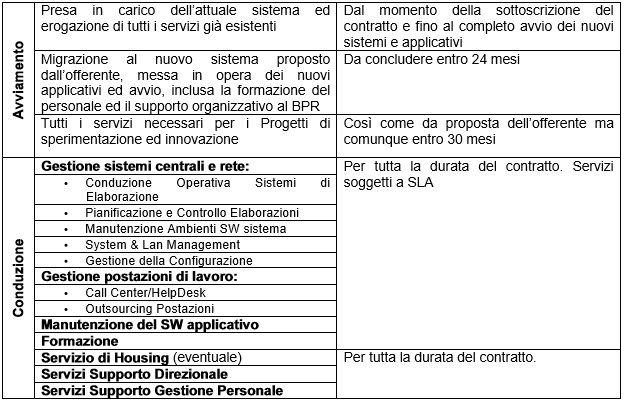
\includegraphics[width=30em]{immagini/sla/planning.png}
\caption{Piano dei servizi di gestione}
\end{figure}

\begin{figure}[H]
\centering
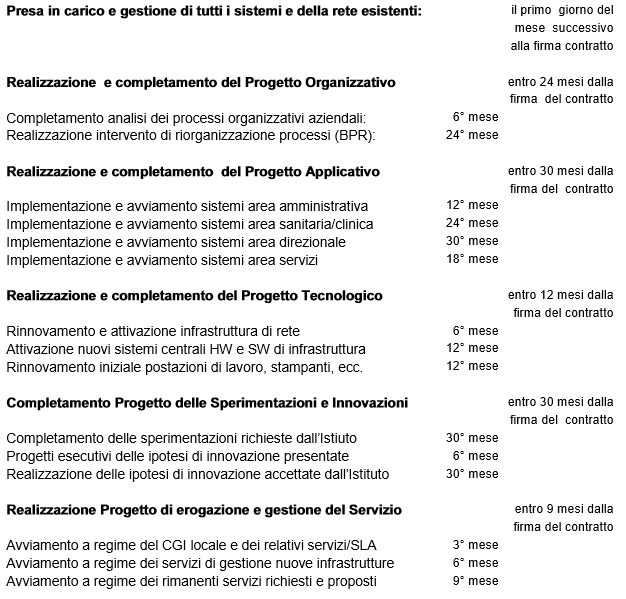
\includegraphics[width=30em]{immagini/sla/timeconstraints.png}
\caption{Vincoli temporali}
\end{figure}

\subsection{Pianificazione delle attività di avviamento}

La seguente tabella illustra le attività di avviamento previste, il periodo di tempo massimo per il loro svolgimento (considerato a partire dalla firma del contratto) e l'obiettivo di riferimento:

\begin{center}
    \begin{tabular}{ | p{4cm} | p{5cm} | l | }
    \hline
    Attività & Obiettivo & Periodo \\ 
    \hline
    
    Formazione & Favorire la comunicazione con i manager tramite una formazione intensiva riguardo ITIL & Entro un mese \\ 
    \hline
    Identificazione dei requisiti di business & Uniformare la visione del business con i processi che coinvolgono il nuovo dipartimento IT & Entro un mese \\ 
    \hline
    Analisi dello stato attuale & Comprendere le caratteristiche e le dinamiche dell'attuale dipartimento IT & Entro due mesi \\
    \hline
    Scelta dei responsabili del processo di SLA Management & Nominare i responsabili e affidare loro le attività riguardanti lo SLA Management & Entro due mesi \\
    \hline
    Implementazione del processo di SLA Management per il Centro di Gestione Integrato & Delineare una bozza funzionante del processo di SLA Management (solo per i servizi necessari al CGI) ed inserirlo tra i processi del nuovo dipartimento IT & Entro tre mesi \\
    \hline
    Gap analysis & Localizzare e risolvere dei gap trovati negli attuali processi che coinvolgono il dipartimento IT & Entro tre mesi \\
    \hline
    Creazione del Service Catalogue & Individuare i servizi IT richiesti ed inserirli nel Service Catalogue & Entro quattro mesi \\
    \hline
    Valutazione degli SLAs, OLAs ed UCs preesistenti & Documentare e monitorare gli SLAs, OLAs ed UCs preesistenti ed in seguito valutarli rispetto alle richieste presenti nel Capitolato Tecnico & Entro cinque mesi \\
    \hline
    Definizione di metriche e KPIs & Formulare metriche e KPIs aggiornati alle nuove richieste e necessità del business & Entro sei mesi \\
    \hline
    Definizione delle modalità di monitoraggio & Istituire gli strumenti per il monitoraggio di metriche e KPIs aggiornati & Entro sei mesi \\
    \hline
    Implementazione del nuovo processo di SLA Management & Finalizzare il processo di SLA Management ed inserirlo tra i processi del nuovo dipartimento IT & Entro otto mesi \\
    \hline
    Inserimento di sperimentazioni e innovazioni nello SLA Management & Estendere il processo di SLA Management ai servizi necessari per il progetto delle sperimentazioni e innovazioni presentato & Entro dieci mesi \\
    \hline
    
    \end{tabular}
\end{center}

\subsection{Pianificazione delle attività di conduzione}

Le attività di conduzione sono:

\begin{itemize}
	\item Establish - Ridefinizione del processo;
    \item Implement - Implementazione dei nuovi SLAs;
    \item Manage - Monitoraggio del processo;
    \item Review - Revisione del processo.
\end{itemize}

%**********************************************************

\section{Attività di avviamento}

\subsection{Formazione}

La formazione necessaria al nuovo processo di SLA Management fa parte dell'introduzione al framework ITIL nell'Azienda Ospedaliera. Sebbene il nuovo dipartimento IT sarà composto da personale qualificato (sia interno che esterno) a nostra discrezione, la logica ITIL non può maturare senza un'espansione verso i dipendenti dell'Istituto stesso. 
\\
Riteniamo indispensabile programmare un corso di formazione sul framework ITIL coinvolgendo ogni manager che lavorerà a contatto con il nuovo dipartimento IT, e sotto gli stessi presupposti lo riteniamo consigliabile anche per gli altri dipendenti. La cooperazione con i manager è fondamentale per ottenere una chiara visione del business e soddisfarne le richieste. La cooperazione con i dipendenti invece è fondamentale per implementare correttamente i processi ed ottenere risultati a livello operativo. L'istituzione di un linguaggio comune costituisce la garanzia a lungo termine per un rapporto virtuoso tra Azienda Ospedaliera e nuovo dipartimento IT, di cui il Capitolato Tecnico costituisce una mera base di partenza.
\\
Dal lato opposto è fondamentale che il business comprenda i vantaggi dell'adozione del framework ITIL, ed in particolare il rigido rispetto degli SLAs così da pubblicizzarli e metterli pienamente a frutto. Il nostro scopo come organizzazione non è solo l'erogazione dei servizi richiesti, ma anche l'inquadramento dei processi preesistenti all'interno dell'Istituto in un'ottica di efficacia, efficienza e miglioramento continuo.
\\ \\
Per l'attività di formazione prevediamo la partecipazione a seminari collettivi al livello ITIL Foundations di figure manageriali e dipendenti scelti. I seminari saranno organizzati da nostri esperti provvisti di certificazione ufficiale.

\subsection{Identificazione dei requisiti di business}

Come accennato nella sezione precedente, il Capitolato Tecnico costituisce una buona base di partenza per identificare i requisiti di business ma è impossibile catturarne la visione completa da un singolo documento. In particolare, evidenzieremo i requisiti di business riguardanti il nuovo processo di SLA Management.
\\
Nel Capitolato Tecnico, alla sezione 5.3 - Definizione Servizi e SLA, si possono consultare i Service Level Requirements rilevati dall'Azienda Ospedaliera. Nel documento sono indicati come Service Level Agreements, ma ci permettiamo di correggere la terminologia. Infatti, gli SLR sono le richieste avanzate dal cliente al fornitore che descrivono le aspettative riguardanti il servizio erogato, esattamente ciò che risulta descritto nel documento. Per definire degli SLAs ottimali è necessario confermare correttezza e completezza degli SRLs già documentati.
\\ \\
Per l'attività di identificazione dei requisiti di business prevediamo di effettuare visite, interviste e riunioni che coinvolgano il personale (principalmente figure manageriali) e le unità di business a stretto contatto con il dipartimento IT.

\subsection{Analisi dello stato attuale}

Allo scopo di pianificare correttamente processi ed attività, riteniamo vitale stabilire lo stato attuale dell'Istituto, in particolare nel settore IT. I fattori più influenti che valuteremo sono:

\begin{itemize}
	\item lo stato dei software (software generici, applicativi specifici dell'Azienda Ospedaliera, criteri e modalità di accesso e download ai software...);
    \item lo stato delle attrezzature hardware (server, desktop, router, periferiche, cavi, giacenze in magazzino...);
    \item la capacità di monitoraggio delle prestazioni attuali (misurazioni sulla connessione internet, misurazioni sulle risposte degli applicativi...);
    \item lo stato del personale ospedaliero (disponibilità fisica e temporale, competenze individuali...);
    \item la presenza di dinamiche interne peculiari (rispetto di procedure e processi, metodi di generazione e trasporto di documentazione, gestione delle emergenze...);
    \item la disponibilità e le caratteristiche degli spazi per il nuovo dipartimento IT (Centro Elaborazione Dati - CED, networking tra le stanze...);
    \item le limitazioni geografiche tra stanze, piani ed edifici (presenza di ostacoli, limitazioni dovute a macchinari medici, distanza geografica elevata...);
    \item la percezione dei servizi erogati dall'Azienda Ospedaliera (dal punto di vista di business/dipendenti/pazienti...);
    \item il grado di maturità del processo preesistente che si occupa degli SLAs (Capability Maturity Model).
\end{itemize}

Per l'attività di analisi dello stato attuale prevediamo la consultazione di documenti preesistenti e l'organizzazione di visite, interviste e riunioni che coinvolgano il personale (principalmente figure manageriali) e le unità di business a stretto contatto con il dipartimento IT.

\subsection{Scelta dei responsabili del processo di SLA Management}

L'assegnazione delle responsabilità ad una persona fisica apre una finestra di dialogo diretto con l'Istituto. Tre sono i ruoli principali che abbiamo individuato:

\begin{itemize}
	\item un Service Level Manager (Process Owner);
    \item almeno un Service Owner;
    \item almeno un Customer Representative.
\end{itemize}

Il Service Level Manager è responsabile della stipulazione e dell'adempimento degli SLAs. Si occupa di garantire la conformità del processo di SLA Management, degli OLAs e degli Underpinning Contracts rispetto agli SLAs. Inoltre, si occupa del monitoraggio e dei documenti di report per gli SLAs.
\\
Il Service Owner è responsabile dell'erogazione di un determinato servizio e spesso ricopre un lato tecnico. Il numero di Service Owners sarà deciso dalla nostra organizzazione in base alle necessità verso la gestione dei servizi preesistenti. Ciascun Service Owner prenderà in carico uno o più servizi e valuterà le attuali prestazioni, proponendo un piano per gli sviluppi futuri (dismissione, delega ad un service provider esterno, erogazione del servizio internamente...).
\\
Il Customer Representative è il rappresentante degli interessi del cliente (in questo caso l'Azienda Ospedaliera). Si occupa di comunicare le aspettative del business verso lo SLA Management grazie alla sua esperienza lavorativa ed alla sua conoscenza del settore ospedaliero. Il numero di Customer Representatives è a discrezione dell'Azienda Ospedaliera, ma consigliamo l'assegnazione di almeno uno di essi così da addolcire l'insediamento del nuovo dipartimento IT.
\\
Per l'attività di scelta dei responsabili del processo di SLA Management prevediamo dunque l'assegnazione dei ruoli di Service Level Manager e Service Owner internamente alla nostra organizzazione, e l'assegnazione del ruolo di Customer Representative internamente all'Azienda Ospedaliera.

\subsection{Implementazione del processo di SLA Management per il Centro di Gestione Integrato}

I vincoli temporali presentati nel Capitolato Tecnico pianificano l'avviamento a regime del Centro di Gestione Integrato locale e di relativi servizi/SLAs entro il terzo mese dopo la firma del contratto. Al fine di rispettarli, la nostra organizzazione definirà una bozza per il nuovo processo di SLA Management riguardante solo i servizi necessari al CGI. La finalizzazione del processo di SLA Management richiede un'analisi più approfondita di quella conducibile in soli tre mesi: questa attività quindi formulerà una versione parziale e temporanea del processo, da estendere e perfezionare successivamente durante l'attività di implementazione del nuovo processo di SLA Management.
\\
Per l'attività di implementazione del processo di SLA Management per il Centro di Gestione Integrato prevediamo l'istituzione di un team di esperti, stabilito internamente alla nostra organizzazione, e dedicato esclusivamente a questa attività.

\subsection{Gap analysis}

La gap analysis è uno strumento manageriale per confrontare le attuali performance del business con quelle potenziali. Con il termine gap si intende l'allocazione non ottimale delle risorse. Approfittando delle circostanze di rinnovamento totale del dipartimento IT, accorceremo la distanza di prospettive tra esso ed il business dell'Istituto. Processi inefficaci, procedure obsolete e sprechi di risorse influiscono enormemente sulle performance dei servizi IT, in particolare la reattività alle segnalazioni.
\\
Per l'attività di gap analysis prevediamo l'istituzione di un team di esperti che abbia a disposizione le informazioni ricavate dall'attività di analisi dello stato attuale. Tale team sarà composto sia da nostri esperti sia da esponenti dell'Azienda Ospedaliera, così da condurre a risultati quanto più accurati possibili.

\subsection{Creazione del Service Catalogue}

Il Service Catalogue è un documento contenente l'elenco dettagliato di tutti i servizi di un fornitore visibili ai clienti. Comprende i servizi di terze parti, in quanto la nostra organizzazione ha la responsabilità riguardo alla loro erogazione ed ai rapporti con i rispettivi fornitori. La prima versione del Service Catalogue comprenderà solo i servizi attualmente erogati, reperibili nel Capitolato Tecnico, sezione 2.2 - Sistemi applicativi esistenti e descrizione del contesto. Formuleremo versioni successive durante le normali attività di conduzione del processo di SLA Management.
\\
Per l'attività di creazione del Service Catalogue prevediamo l'istituzione di un team di esperti, stabilito internamente alla nostra organizzazione.

\subsection{Valutazione degli SLAs, OLAs ed UCs preesistenti}

Gli attuali servizi erogati all'Istituto, qualunque siano i rispettivi fornitori, dovrebbero rispettare determinati SLAs che possibilmente saranno a loro volta alimentati da OLAs ed UCs con terze parti. Valutare le condizioni attuali dei servizi è imperativo per garantire gli SLAs richiesti nel Capitolato Tecnico. Qualora uno o più servizi non rispettassero i nuovi SLAs mantenendo gli attuali contratti, la nostra organizzazione si farà carico di risolvere la situazione.
\\
Per l'attività di valutazione degli SLAs, OLAs ed UCs preesistenti prevediamo l'istituzione di un team di esperti, stabilito internamente alla nostra organizzazione.

\subsection{Definizione di metriche e KPIs}

I KPIs sono quantità misurabili di natura strategica che riflettono la vicinanza del business ai propri obiettivi. In quanto tali, la scelta di essi è strettamente influenzata dalla visione del business; di cui saremo a conoscenza grazie alle attività di identificazione dei requisiti di business e di gap analysis.
\\
Le metriche sono quantità misurabili di natura tattica che riflettono le performance di processi/attività. In quanti tali, la scelta di esse è strettamente influenzata dal processo/attività di riferimento. Nell'ambito del processo di SLA Management, le metriche provengono dagli SLAs richiesti nel Capitolato Tecnico nonchè dagli OLAs ed UCs preesistenti; di cui siamo a conoscenza grazie alle attività di analisi dello stato attuale, di creazione del Service Catalogue e di valutazione degli SLAs, OLAs ed UCs preesistenti.
\\
Per l'attività di definizione di metriche e KPIs prevediamo l'istituzione di un team di esperti, stabilito internamente alla nostra organizzazione.

\subsection{Definizione delle modalità di monitoraggio}

Le modalità di monitoraggio dipendono strettamente dalle metriche e dai KPIs stabiliti per il processo di SLA Management. La chiara definizione di metriche e KPIs dunque è un prerequisito fondamentale per questa attività. Il monitoraggio deve tener conto anche degli elementi software ed hardware a disposizione, così da fornire la soluzione ottimale con le risorse attualmente a disposizione. Redigeremo un elenco delle possibli migliorie e criticità, con una valutazione riguardo a costi e benefici.
\\
Per l'attività di definizione delle modalità di monitoraggio prevediamo l'istituzione di un team di esperti, stabilito internamente alla nostra organizzazione.

\subsection{Implementazione del nuovo processo di SLA Management}

A partire dai processi interni all'Istituto, in particolare quelli che si interfacceranno con il nuovo dipartimento IT, applicheremo gradualmente i cambiamenti dettati dalla logica ITIL e dal business. Al termine di questa lenta metamorfosi, i processi saranno stati completamente rinnovati e riorganizzati.
\\
Il processo di SLA Management entrerà nel pieno delle attività di conduzione seguendo uno pseudociclo (Establish, Implement, Manage e Review). Istanzieremo i sottoprocessi dello SLA Management (Maintenance of the SLM Framework, Identification of Service Requirements, Agreements Sign-Off and Service Activation e Service Level Monitoring and Reporting) e abiliteremo operativamente il rispettivo personale. Sostituiremo la versione temporanea del processo di SLA Management ristretta al Centro di Gestione Integrato con la versione completa, rielaborata con più cura durante i mesi trascorsi.
\\
Per l'attività di definizione delle modalità di monitoraggio prevediamo l'istituzione di un team di esperti, stabilito internamente alla nostra organizzazione, e dedicato esclusivamente a questa attività.

\subsection{Inserimento di sperimentazioni e innovazioni nello SLA Management}

I vincoli temporali presentati nel Capitolato Tecnico prevedono la presentazione dei progetti esecutivi delle ipotesi di innovazione presentate entro il sesto mese dalla firma del contratto. Considerato ciò, preferiamo finalizzare il nuovo processo di SLA Management e verificarne le performance prima di dedicarci alle sperimentazioni ed innovazioni. Una volta delineati i progetti esecutivi delle ipotesi di innovazione, condurremo analisi e valutazioni del loro possibile impatto sui processi del nuovo dipartimento IT, prima di procedere con l'inserimento nel processo di SLA Management.
\\
Per l'attività di inserimento di sperimentazioni e innovazioni nello SLA Management prevediamo l'utilizzo di risorse già previste per le normali attività di conduzione dal processo di SLA Management.

%**********************************************************

\section{Attività di conduzione}

\subsection{Establish - Ridefinizione del processo}

Durante l'attività di Establish (e solo durante essa) apportiamo eventuali cambiamenti al processo, approvati da una precedente attività di Review. Fattori scatenanti possono essere variazioni degli SLAs, delle strategie di business, dei Service Improvement Programs oppure semplicemente ottimizzazioni a livello operativo ed organizzativo. Questa attività pianifica ed organizza il futuro del processo di SLA Management delineandone l'evoluzione, gli obiettivi e le prossime milestones.

\subsection{Implement - Implementazione dei nuovi SLAs}

Durante l'attività di Implement delineiamo e progressivamente limiamo le bozze di SLAs, OLAs ed UCs, fino ad ultimare i contratti ufficiali con i clienti. Parallelamente studiamo la fattibilità ed i costi degli SLAs richiesti, ridimensionandoli secondo i bisogni del cliente o dell'Azienda Ospedaliera. Nel caso della pubblicazione o del ritiro di un servizio, aggiorniamo puntualmente il Service Catalogue.


\subsection{Manage - Monitoraggio del processo}

Durante l'attività di Manage monitoriamo le performance dei servizi secondo le metriche ed i KPIs prestabiliti. Valutiamo e successivamente archiviamo i rilievi sulle performance, così da possedere in futuro una visione dei servizi sull'asse temporale. Inoltre stiliamo periodicamente i report per i vari servizi e qualora ritenuto necessario possiamo indire un incontro di review per determinati servizi.


\subsection{Review - Revisione del processo}

Durante l'attività di Review indiciamo periodicamente le review dei servizi ed elaboriamo i Service Improvement Programs riguardanti il processo di Continual Service Improvement. L'adozione di metriche e KPIs significativi ha particolamente influenza sull'attività di Review, che si basa ampiamente sugli output dell'attività di Manage sia per le review che per la scrittura dei SIPs.


%**********************************************************

\section{Strumenti software a supporto del processo di SLA Management}

Gli obiettivi dell'Istituto rispetto agli SLAs sono:

\begin{itemize}
	\item il continuo monitoraggio di informazioni riguardanti metriche e KPIs;
	\item la possibilità di analizzare le informazioni di monitoraggio;
    \item la presenza di un sistema aperto che favorisca lo scambio delle informazioni di monitoraggio.
\end{itemize}

Il nuovo processo di SLA Management garantirà un livello di dettaglio e controllo estremamente più preciso, penetrante ed approfondito rispetto al passato. Per questo motivo è necessario adottare nuovi strumenti software specializzati in tali compiti, supportati da elementi hardware adeguati.
\\
Data la complessità delle operazioni per istanziare il nuovo processo di SLA Management e le tempistiche ristrette, abbiamo ritenuto più vantaggioso adottare strumenti differenti prima a supporto delle attività di avviamento e poi a supporto delle attività di conduzione.


\subsection{Strumenti software a supporto delle attività di avviamento}

Durante le attività di avviamento, la maggior parte dei servizi è ancora erogata da fornitori di terze parti e non internamente al dipartimento IT: ne consegue un debole controllo del monitoraggio e la quasi impossibilità di scambio di dati tra i vari servizi. Delineare una soluzione definitiva così presto, prima ancora di terminare le analisi preliminari, valutare la situazione e stabilire la visione del business, sarebbe decisamente sconsiderato e dannoso a lungo termine. La nostra organizzazione possiede una partnership commerciale con Uptrends, specializzato in qualsiasi genere di strumenti per il monitoraggio via software. Uptrends spicca per la sua assoluta indipendenza da qualsiasi servizio/applicazione/piattaforma si voglia monitorare. Grazie ad esso siamo in grado di creare una struttura informatica provvisoria ed economica adatta al monitoraggio degli SLAs in poche settimane.

\subsubsection{Uptrends - Website Uptime Monitoring}

\begin{figure}[H]
\centering
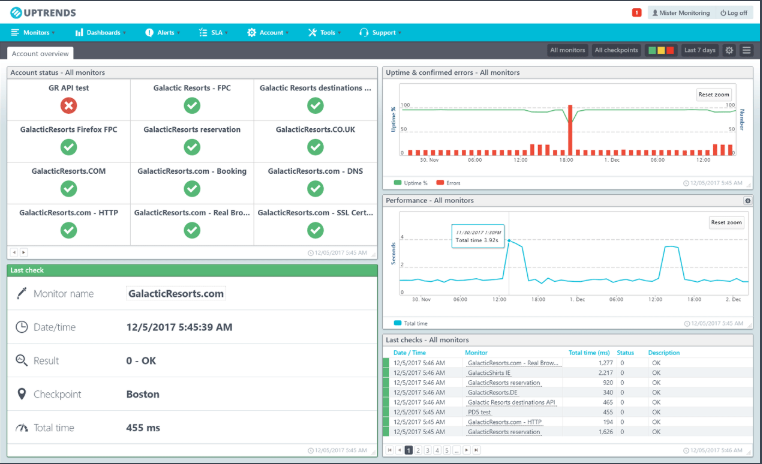
\includegraphics[width=30em]{immagini/sla/websitemonitor.png}
\caption{Schermata esemplificativa di Uptrends - Website Uptime Monitoring}
\end{figure}

Questo strumento software permette di monitorare:

\begin{itemize}
	\item le richieste HTTP/HTTPS;
    \item i webservice (SOAP, REST API);
    \item i certificati SSL;
    \item i DNS;
    \item i server.
\end{itemize}

Viene utilizzato principalmente durante le attività di valutazione dello stato attuale e di valutazione degli SLAs, OLAs ed UCs preesistenti. La velocità di installazione e la comodità d'uso sono controbilanciate dalla scarsa profondità delle informazioni ricavate, che comunque corrispondono adeguatamente alle necessità del nuovo dipartimento IT durante i primi mesi dalla firma del contratto. Per ulteriori informazioni riguardo ad Uptrends - Website Uptime Monitoring consultare la sezione \href{https://www.uptrends.com/products/website-monitoring}{Website Monitoring} presente nel sito web di Uptrends.
\\
Uptrends - Website Uptime Monitoring verrà sostituito il prima possibile (idealmente entro cinque mesi) con analoghi moduli presenti in SAP Solution Manager - IT Service Management.

\subsubsection{Uptrends - API Monitoring}

\begin{figure}[H]
\centering
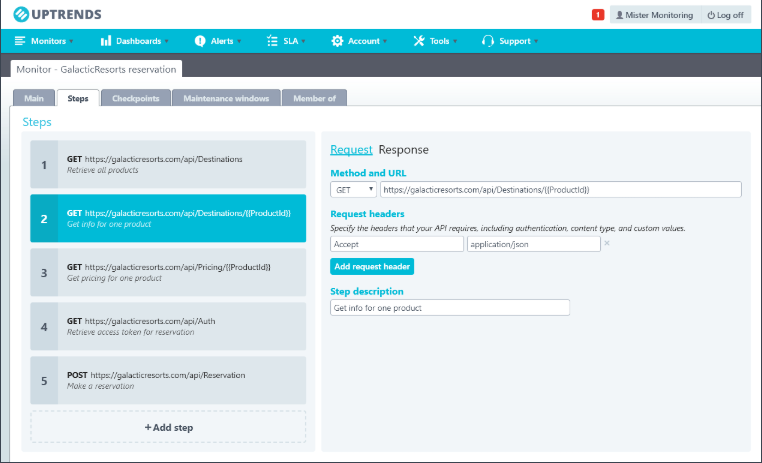
\includegraphics[width=30em]{immagini/sla/apimonitor.png}
\caption{Schermata esemplificativa di Uptrends - API Monitoring}
\end{figure}

Questo strumento software permette di monitorare:

\begin{itemize}
	\item le situazioni con chiamate API multiple;
    \item il corretto funzionamento delle API;
    \item il downtime delle API per il calcolo degli SLAs;
    \item il rispetto dei tempi massimi di risposta delle API;
    \item gli avvisi in caso di malfunzionamento delle API.
\end{itemize}

Viene utilizzato principalmente durante le attività di valutazione degli SLAs, OLAs ed UCs preesistenti e di definizione delle modalità di monitoraggio. L'installazione e la configurazione possono presentare qualche difficoltà nel caso in cui le API non siano ben strutturate e documentate, ma le informazioni ricavate sono dettagliate e facilmente personalizzabili. La possibilità di effettuare controlli continui permette una notevole tempestività da parte del nuovo dipartimento IT fin dai primi mesi dopo il suo insediamento. Per ulteriori informazioni riguardo ad Uptrends - API Monitoring consultare la sezione \href{https://www.uptrends.com/solutions/api-monitoring}{Multi-step API Monitoring} presente nel sito web di Uptrends.
\\
Uptrends - API Monitoring verrà sostituito solo all'avvento della versione finale del processo di SLA Management (idealmente entro otto mesi) con analoghi moduli presenti in SAP Solution Manager - IT Service Management.

\subsubsection{Uptrends - External Server Monitoring}

\begin{figure}[H]
\centering
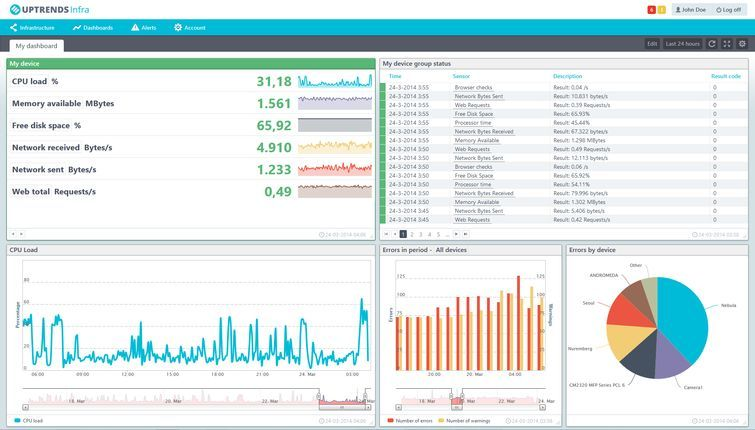
\includegraphics[width=30em]{immagini/sla/servermonitor.png}
\caption{Schermata esemplificativa di Uptrends - External Server Monitoring}
\end{figure}

Questo strumento software permette di monitorare:

\begin{itemize}
	\item i server di posta elettronica;
    \item i database SQL;
    \item i webserver.
\end{itemize}

Viene utilizzato principalmente durante le attività di valutazione dello stato attuale e di valutazione degli SLAs, OLAs ed UCs preesistenti. Gli elementi monitorati sono esclusivamente di dominio interno al nuovo dipartimento IT (dunque non riguardanti i servizi erogati da terze parti) così da garantire la stabilità dei sistemi informatici nelle situazioni di ordinaria amministrazione. Per ulteriori informazioni riguardo ad Uptrends - External Server Monitoring consultare la sezione \href{https://www.uptrends.com/products/external-server-monitoring}{External Server Monitoring} presente nel sito web di Uptrends.
\\
Uptrends - External Server Monitoring verrà sostituito durante l'implementazione del processo di SLA Management (idealmente entro sette mesi) con analoghi moduli presenti in SAP Solution Manager - IT Service Management.

\subsubsection{SAP Solution Manager - IT Service Management}

\begin{figure}[H]
\centering
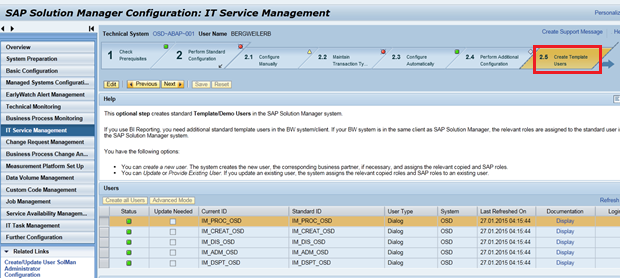
\includegraphics[width=30em]{immagini/sla/itservicemanagement.png}
\caption{Schermata esemplificativa di SAP Solution Manager - IT Service Management}
\end{figure}

Questo strumento software permette di automatizzare ogni aspetto relativo agli SLAs dei servizi erogati dal nuovo dipartimento IT. In particolare risolve i seguenti punti chiave per il nuovo processo di SLA Management:

\begin{itemize}
	\item la creazione di servizi e profili di risposta;
	\item la configurazione generica del processo di SLA Management;
	\item la definizione delle procedure per il rilevamento degli SLAs nei vari casi d'uso;
	\item la configurazione della procedure di escalation, permettendone anche l'invio di notifiche attraverso email;
	\item la definizione di specifiche caratteristiche per il monitoraggio ed il reporting degli SLAs.
\end{itemize}

In quanto la gestione degli SLAs sarà interamente automatizzata, la corretta configurazione di questo software sarà estremamente importante, nonchè lunga e delicata. Per illustrare il funzionamento di SAP Solution Manager - IT Service Management, presentiamo sinteticamente un caso d'uso esemplificativo: la gestione degli SLAs in occasione di un incidente relativo ad un configuration item fornito da un venditore di hardware.
\\ \\
Dopo aver effettuato l'accesso al proprio sistema SAP, si ha accesso alla schermata di SAP Solution Manager IT Service Management. Visualizzando l'incidente, si può verificare come il venditore di hardware ed il codice del configuration item siano stati rilevati automaticamente dal software.

\begin{figure}[H]
\centering
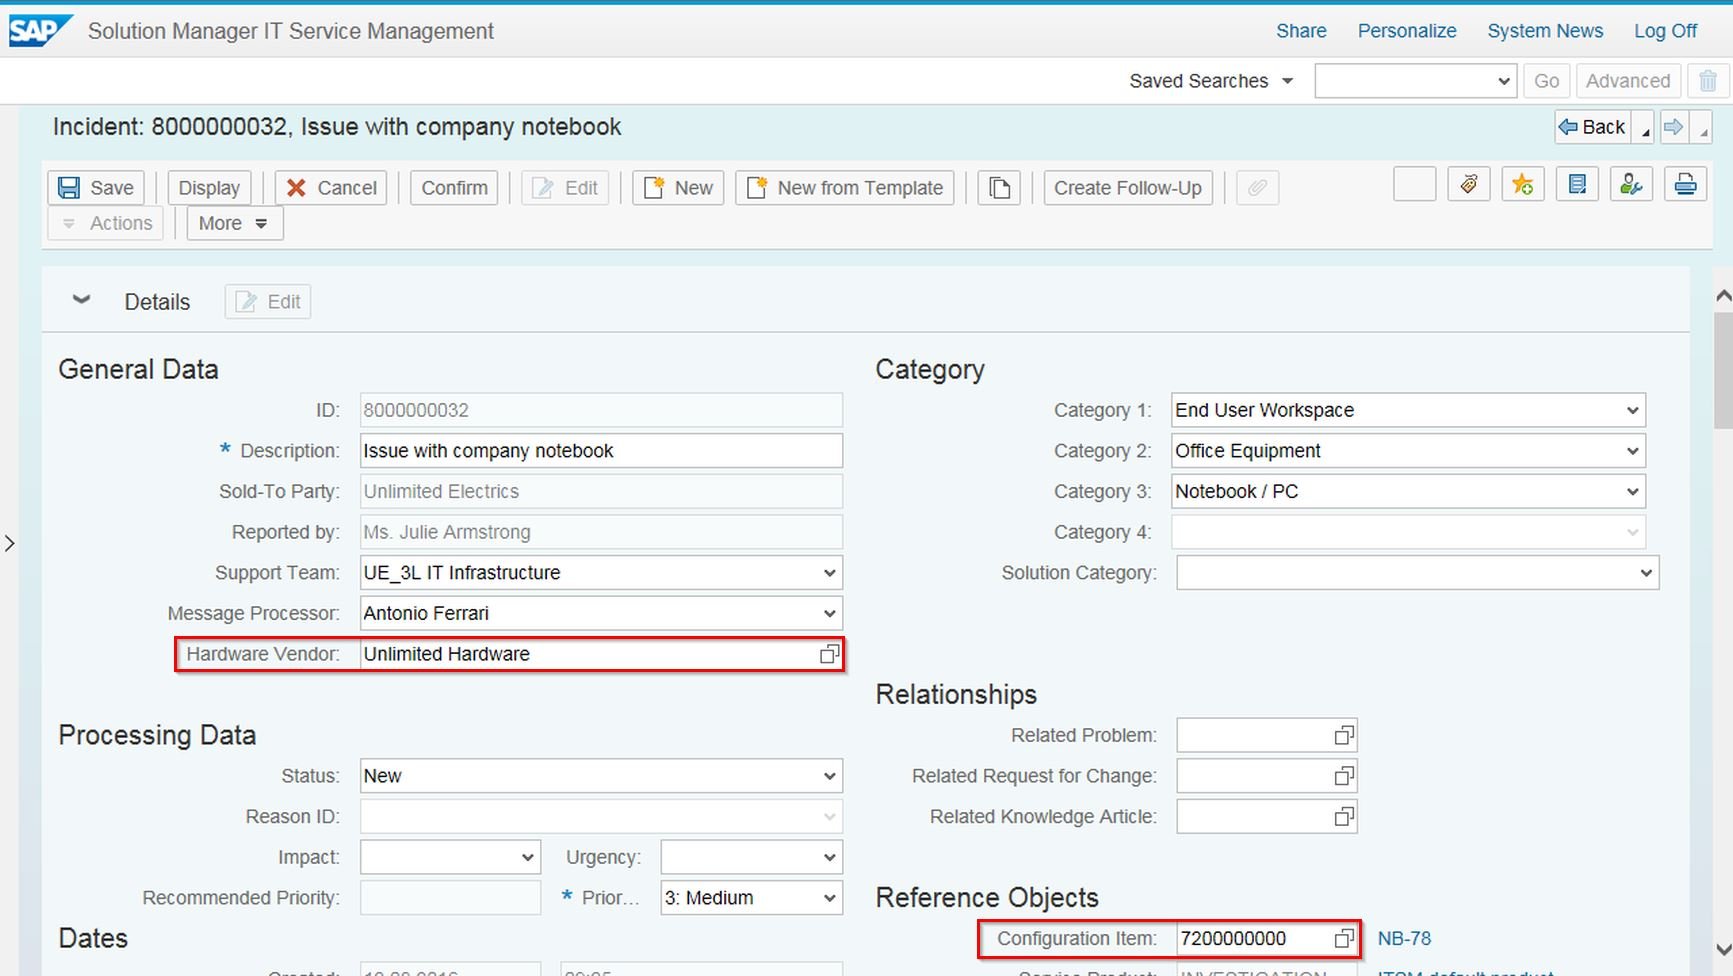
\includegraphics[width=30em]{immagini/sla/sm1.png}
\caption{Caso d'uso - Visualizzazione dell'incidente}
\end{figure}

I tempi operativi per OLAs ed UCs risultano non calcolati, infatti non è stato ancora stabilito lo status dell'incidente.

\begin{figure}[H]
\centering
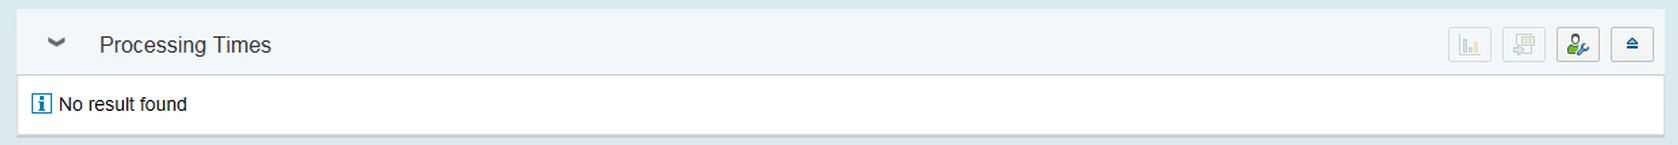
\includegraphics[width=30em]{immagini/sla/sm2.png}
\caption{Caso d'uso - Visualizzazione dei tempi di OLAs ed UCs}
\end{figure}

Appena il dipartimento IT definisce lo status dell'incidente, cioè un difetto nell'hardware, questo viene aggiornato. Il software rileva un contratto attivo con il venditore di hardware, lo notifica ed inizia il calcolo dei parametri concordati nell'UC con tale venditore.

\begin{figure}[H]
\centering
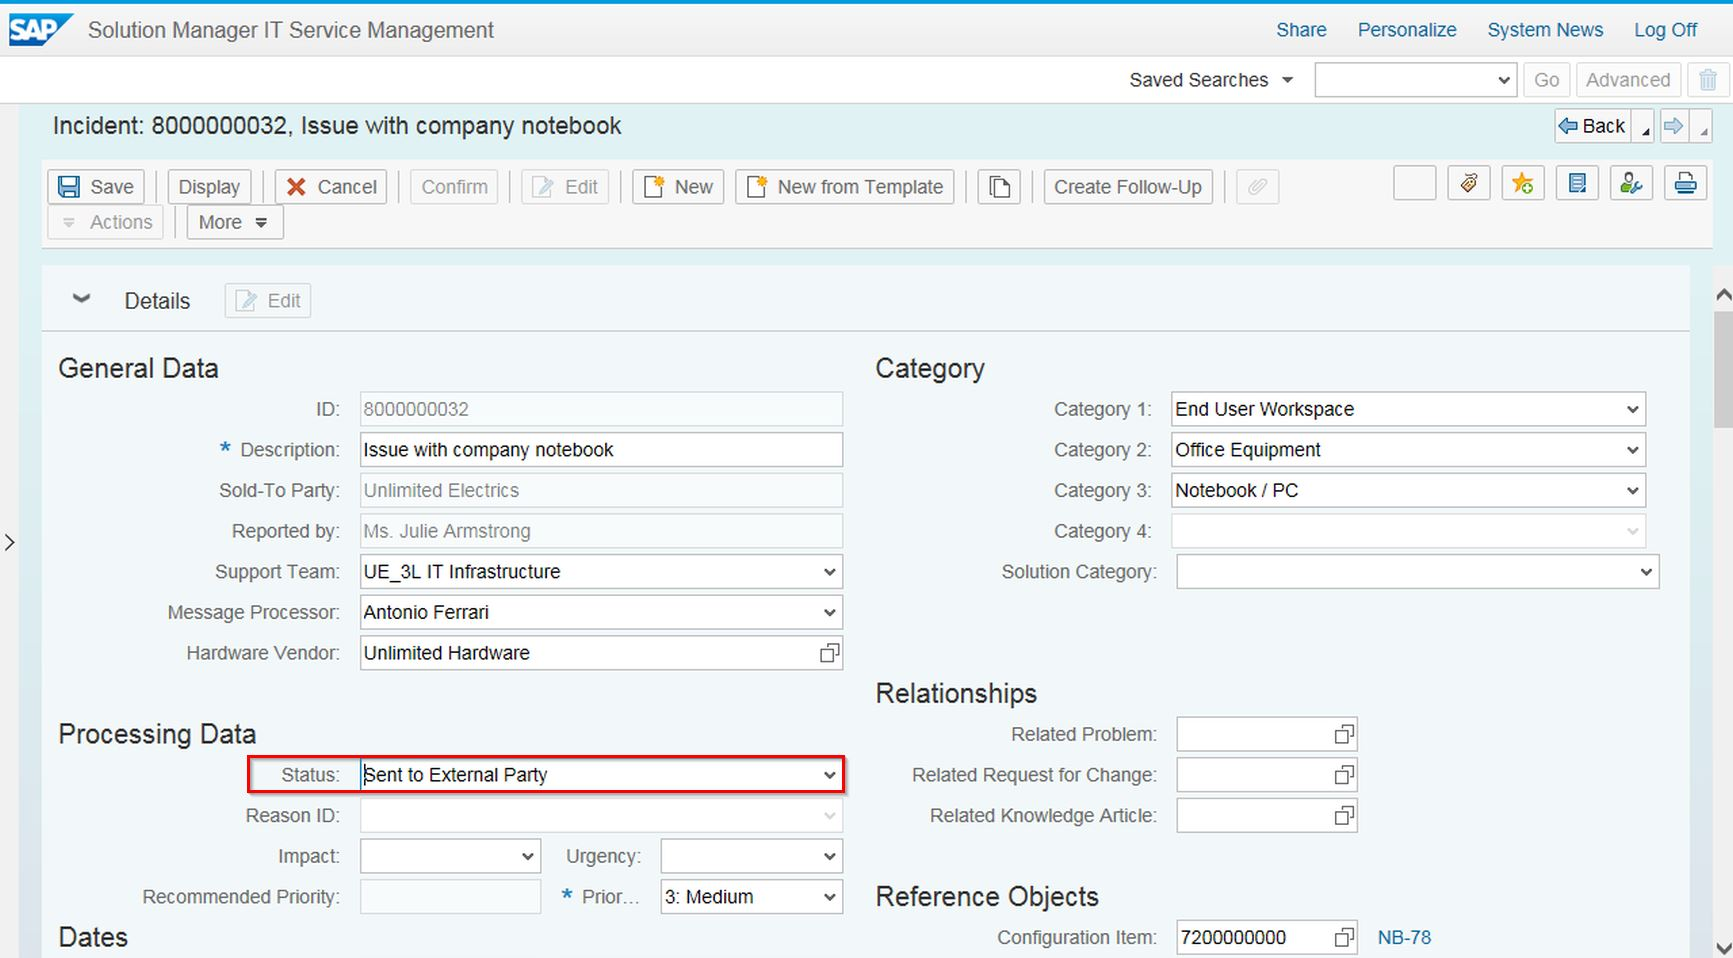
\includegraphics[width=30em]{immagini/sla/sm3.png}
\caption{Caso d'uso - Aggiornamento dello status dell'incidente}
\end{figure}

I tempi operativi per l'UC con il venditore di hardware sono inizializzati e calcolati.

\begin{figure}[H]
\centering
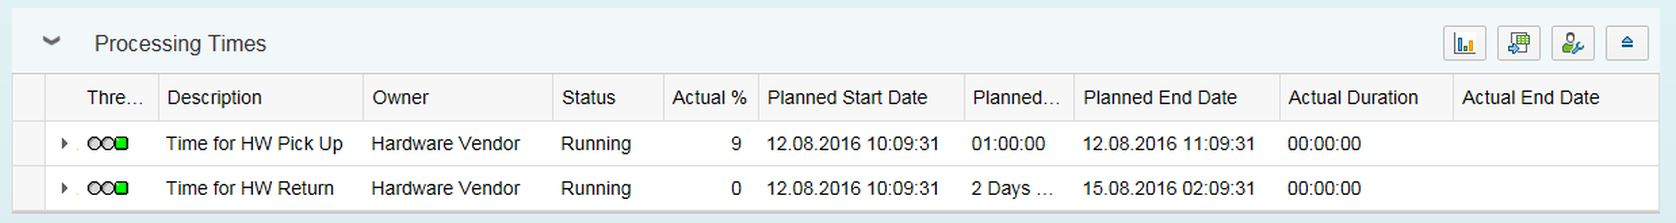
\includegraphics[width=30em]{immagini/sla/sm4.png}
\caption{Caso d'uso - Visualizzazione dei tempi di OLAs ed UCs aggiornati}
\end{figure}

Quando l'hardware viene riparato e riconsegnato, e dunque l'incidente viene chiuso, si possono visualizzare le tempistiche del venditore di hardware ed il loro rispetto delle soglie concordate nell'UC.

\begin{figure}[H]
\centering
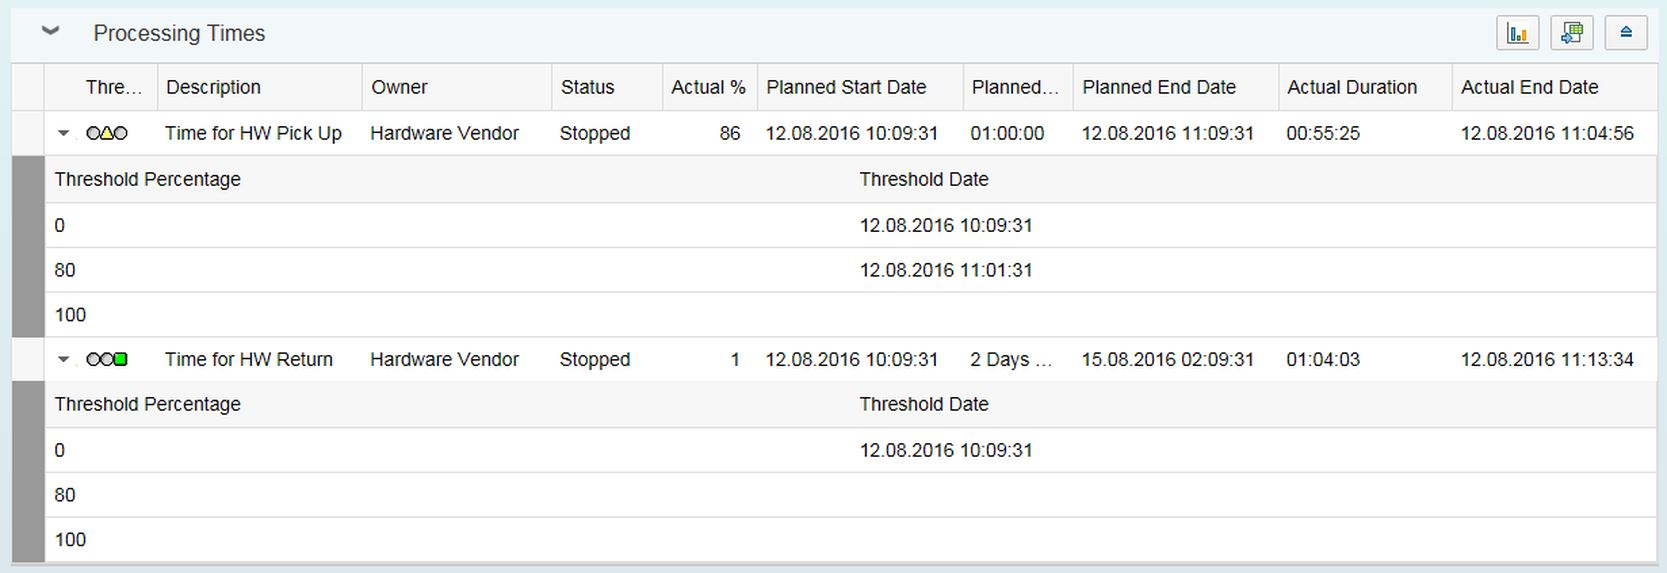
\includegraphics[width=30em]{immagini/sla/sm5.png}
\caption{Caso d'uso - Visualizzazione delle soglie temporali per l'UC}
\end{figure}

Per ogni servizio erogato all'Azienda Ospedialiera, la nostra organizzazione vuole raggiungere un simile livello di automatizzazione e dettaglio. Per ulteriori informazioni riguardo a SAP Solution Manager - IT Service Management consultare la sezione \href{https://wiki.scn.sap.com/wiki/display/SAPITSM/Service+Level+Management}{Service Level Management} presente nella community wiki di SAP Solution Manager.

\subsubsection{SAP Solution Manager - Service Desk}

\begin{figure}[H]
\centering
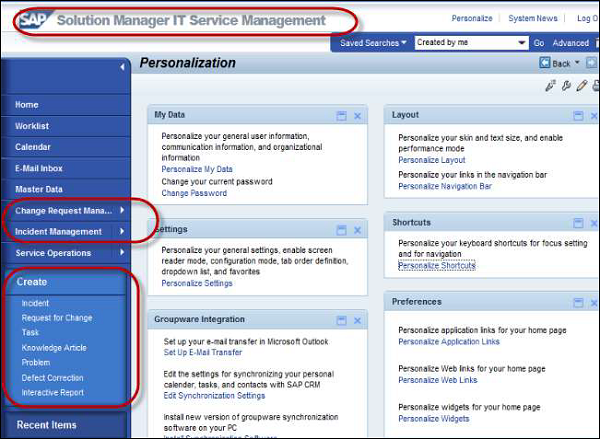
\includegraphics[width=30em]{immagini/sla/servicedesk.png}
\caption{Schermata esemplificativa di SAP Solution Manager - Service Desk}
\end{figure}

Questo strumento software permette principalmente di gestire incidenti e service requests, garantendo l'adeguato livello di supporto agli utenti. Per illustrare il funzionamento di SAP Solution Manager - Service Desk, presentiamo sinteticamente un caso d'uso esemplificativo: la creazione e la gestione di un ticket.
\\ \\
Dopo aver effettuato l'accesso al proprio sistema SAP, si ha accesso al menù SAP Easy Access. Dal menù Help > Create Support Message si può passare alla compilazione del ticket. Possono essere specificati parametri come le componenti affette, la priorità, il tipo ed i commenti.

\begin{figure}[H]
\centering
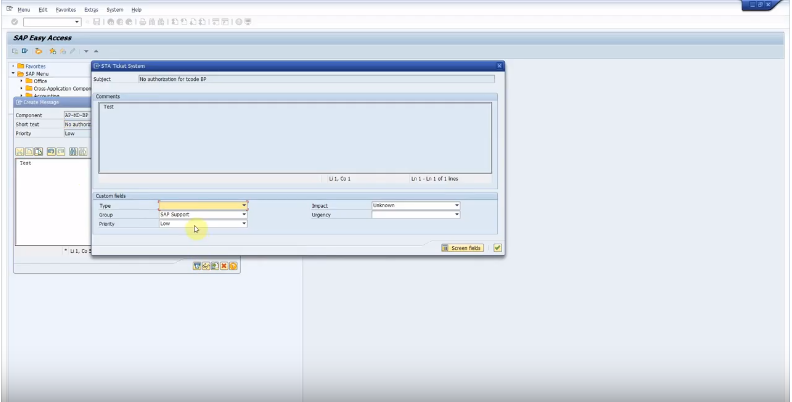
\includegraphics[width=30em]{immagini/sla/sd1.png}
\caption{Caso d'uso - Creazione del ticket}
\end{figure}

Una volta terminata la compilazione, compare un messaggio di invio con successo nel sistema di ticketing.

\begin{figure}[H]
\centering
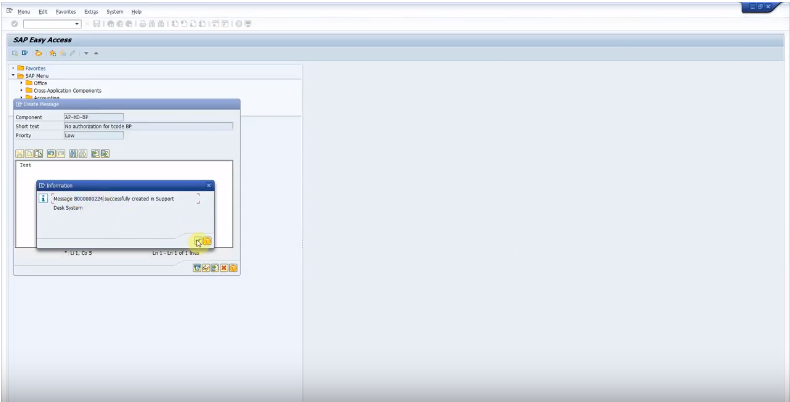
\includegraphics[width=30em]{immagini/sla/sd2.png}
\caption{Caso d'uso - Conferma ed invio del ticket}
\end{figure}

Per creare un incidente a partire dal messaggio di supporto, si deve accedere al Transaction Monitor, per poi eseguire una transazione con il codice corrispondente a quello assegnato al messaggio di supporto.

\begin{figure}[H]
\centering
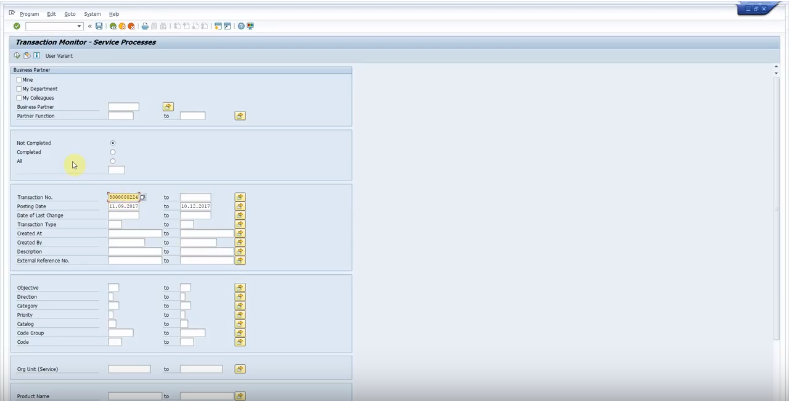
\includegraphics[width=30em]{immagini/sla/sd3.png}
\caption{Caso d'uso - Creazione dell'incidente}
\end{figure}

Il nuovo ticket sarà ora visibile nella schermata di Transaction Monitor.

\begin{figure}[H]
\centering
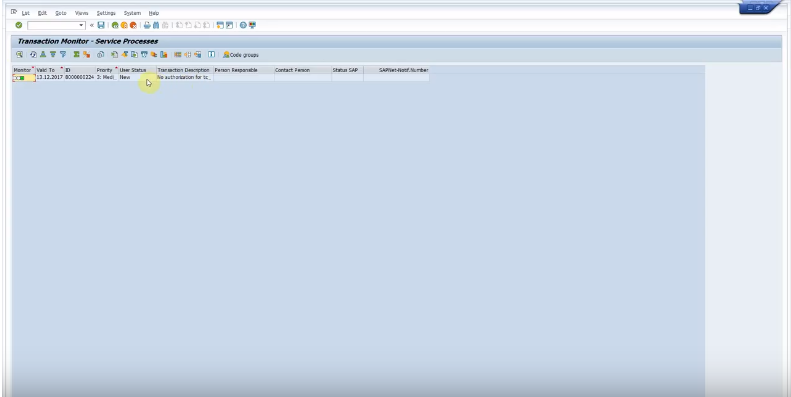
\includegraphics[width=30em]{immagini/sla/sd4.png}
\caption{Caso d'uso - Visualizzazione del ticket nella coda}
\end{figure}

Tra le varie informazioni dettagliate riguardo all'incidente, sarà disponibile automaticamente anche un report in formato pdf.

\begin{figure}[H]
\centering
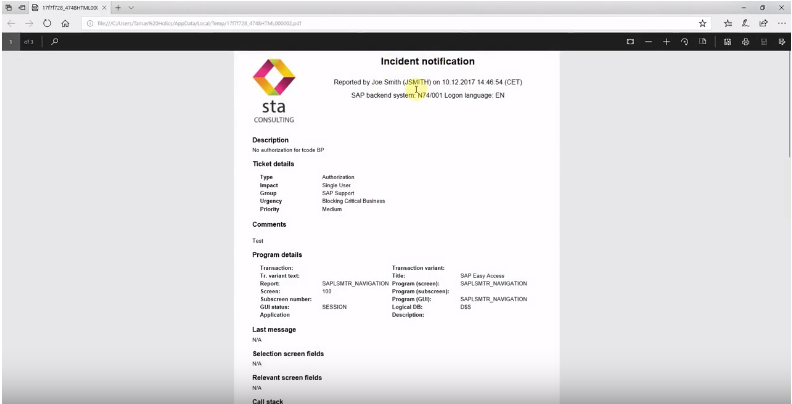
\includegraphics[width=30em]{immagini/sla/sd5.png}
\caption{Caso d'uso - Report dell'incidente}
\end{figure}

Certamente l'uso del software SAP Solution Manager - Service Desk non si riduce al semplice caso d'uso qui presentato. Per ulteriori informazioni riguardo a SAP Solution Manager - Service Desk consultare la sezione \href{https://support.sap.com/en/solution-manager/solution-manager-71/processes-71/it-service-management.html}{IT Service Management} presente in SAP Support Portal.

\subsubsection{Soluzione ad hoc - Interfaccia SLA Manager}

\begin{figure}[H]
\centering
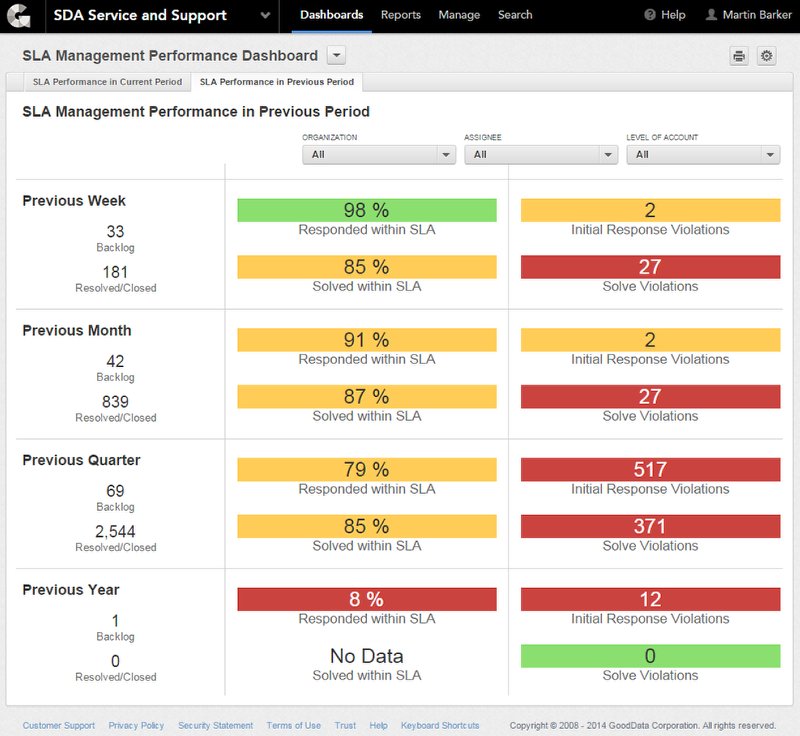
\includegraphics[width=30em]{immagini/sla/slainterface.png}
\caption{Schermata esemplificativa della soluzione ad hoc di interfaccia SLA Manager}
\end{figure}

Come definito nel Capitolato Tecnico, sezione 5.1.4.5 - Misurazione dei livelli di servizio (SLA Management), il sistema informativo dedicato alla gestione degli SLA viene denominato SLA Manager. Durante le attività di avviamento sarà disponibile una soluzione ad hoc provvisoria, consultabile attraverso un'interfaccia semplificata. Gli strumenti software di Uptrends risultano troppo tecnici per il personale non specializzato nell'ambito informatico. La nostra organizzazione ha definito un template standard per riunire tutte le informazioni rilevate dai vari strumenti ed unificarle in un'interfaccia user-friendly. Durante le attività di analisi dello stato attuale e scelta dei responsabili del processo di SLA Management, sono stati definiti specifici gruppi di utenti che potranno consultare ad esempio:

\begin{itemize}
	\item da un singolo servizio all'intero Service Catalogue;
    \item dal semplice stato online/offline alle varie metriche e KPIs monitorati;
    \item dalle informazioni in tempo reale a quelle documentati nei periodi passati.
\end{itemize}

Sebbene durante le attività di avviamento questa soluzione ad hoc sarà ancora provvisoria e probabilmente soggetta a variazioni, riteniamo sia un'ottima scelta anche successivamente all'implementazione del nuovo processo di SLA Management. In tal modo, anche quando la migrazione totale a SAP Solution Manager sarà ultimata, il personale non noterà alcun cambiamento sostanziale nell'interfaccia. Inoltre questo strumento, essendo sviluppato internamente alla nostra organizzazione, potrà adattarsi alle necessità future dell'Istituto e garantire un alto grado di flessibilità.

\subsection{Strumenti software a supporto delle attività di conduzione}

Durante le attività di conduzione, la gestione dei servizi sarà stabile e ben definita (siano essi erogati internamente al nuovo dipartimento IT oppure da fornitori di terze parti). Tutti i servizi interni saranno strettamente collegati al software SAP Solution Manager, dando così vita ad un sistema informativo centralizzato (etichettato come "SLA Manager" nel Capitolato Tecnico). Tutti i servizi esterni dovranno ugualmente essere compatibili e collegati al software SAP Solution Manager, in caso contrario dovranno essere migrati internamente al nuovo dipartimento IT. SAP Solution Manager è uno strumento software estremamente complesso e ramificato, che necessita di tempo per le operazioni di installazione, configurazione e rilascio. Grazie alla sua modularità, alcune sue funzionalità sono state già integrate con il nuovo processo di SLA Management durante le attività di avviamento. L'integrazione dei restanti moduli verrà effettuata durante le attività di conduzione in maniera graduale, in base alla pianificazione precedentemente elaborata.
\\
Segue una breve spiegazione delle funzionalità e dei moduli chiave necessari al processo di SLA Management.

\subsubsection{SAP Solution Manager - IT Service Management}

Questo strumento software sarà già stato utilizzato durante le attività di avviamento, in quanto offre un'ampia gamma di funzionalità indispensabili. I casi d'uso in cui verrà impiegato saranno gradualmente estesi, fino a coprire la quasi interezza (escludendo l'interfaccia) del nuovo sistema informativo, lo SLA Manager. Le principali funzionalità che integreremo nello SLA Manager saranno:

\begin{itemize}
	\item Incident Management, ovvero la gestione degli incidenti;
    \item Problem Management, ovvero la gestione dei problemi;
    \item Request Fulfillment, ovvero la gestione delle Service Request;
    \item Change Request, ovvero la gestione delle richiesti di modifiche ai servizi;
    \item Service Catalogue Management, ovvero la gestione dei cambiamenti apportati al Service Catalogue.
\end{itemize}

Per ulteriori informazioni riguardo a SAP Solution Manager - IT Service Management consultare la sezione \href{https://support.sap.com/en/solution-manager/solution-manager-71/processes-71/it-service-management.html}{IT Service Management} presente in SAP Support Portal, nonchè le sezioni \href{https://wiki.scn.sap.com/wiki/display/SAPITSM/IT+Service+Management+Wiki+for+User}{IT Service Management for User} e \href{https://wiki.scn.sap.com/wiki/display/SAPITSM/ITSM+Wiki+for+Administrator}{IT Service Management for Administrator} presenti nella community wiki di SAP Solution Manager.
\\
Per approfondire l'implementazione del processo di Incident Management in SAP Solution Manager consultare la sezione \href{https://wiki.scn.sap.com/wiki/display/SM/Incident+Management+Overview}{Incident Management} presente nella community wiki di SAP Solution Manager.
\\
Per approfondire l'implementazione del processo di Incident Management in SAP Solution Manager consultare la sezione \href{https://help.sap.com/viewer/0611cd2e5d1e403c9ee7b6efad89e81b/7.2.07/en-US/1f35fb5cda804e71bfcf5c00326eb1fa.html}{Problem Management} presente in SAP Help Portal.
\\
Per approfondire l'implementazione del processo di Request Fulfillment in SAP Solution Manager consultare la sezione \href{https://wiki.scn.sap.com/wiki/display/SAPITSM/Service+Request+Management+Service+Request+Fulfillment}{Service Request Fulfillment} presente nella community wiki di SAP Solution Manager.
\\
Per approfondire l'implementazione del processo di Change Request Management in SAP Solution Manager consultare la sezione \href{https://wiki.scn.sap.com/wiki/display/SM/Change+Request+Management+Overview}{Change Request Management} presente nella community wiki di SAP Solution Manager.
\\
Per approfondire l'implementazione del processo di Service Catalogue Management in SAP Solution Manager consultare la sezione \href{https://wiki.scn.sap.com/wiki/display/SAPITSM/Service+Catalogue+Management}{Service Catalogue Management} presente nella community wiki di SAP Solution Manager.

\subsubsection{SAP Solution Manager - Monitoring}

SAP Solution Manager abilita funzionalità di:

\begin{itemize}
	\item System Monitoring, cioè il monitoraggio di elementi informatici come istanze, database ed host;
    \item Connection Monitoring, cioè il monitoraggio delle connessioni presenti nel proprio sistema informatico;
    \item Business Intelligence Monitoring, cioè il monitoraggio della corretta esecuzione delle operazioni effettuate nel proprio sistema informatico e la generazione di report su di esse;
    \item Process Integration Monitoring, cioè il monitoraggio dell'integrazione tra diversi componenti del proprio sistema informatico;
    \item End-User Experience Monitoring, cioè il monitoraggio di performance ed availability del proprio sistema informatico rispetto ai vari punti di contatto disponibili.
\end{itemize}

Per ulteriori informazioni riguardo a SAP Solution Manager - System Monitoring consultare le sezioni \href{https://wiki.scn.sap.com/wiki/display/TechOps/Solution+Manager+7.2+-+System+Monitoring}{System Monitoring} e \href{https://wiki.scn.sap.com/wiki/display/TechOps/System+Monitoring+7.2+-+Advanced+Monitoring}{Advanced Monitoring} presenti nella community wiki di SAP Solution Manager.
\\
Per ulteriori informazioni riguardo a SAP Solution Manager - Connection Monitoring consultare la sezione \href{https://wiki.scn.sap.com/wiki/display/TechOps/Interface+and+Connection+Monitoring+Setup+with+SAP+Solution+Manager+7.2}{Interface and Connection Monitoring Setup} presente nella community wiki di SAP Solution Manager.
\\
Per ulteriori informazioni riguardo a SAP Solution Manager - Business Intelligence Monitoring consultare la sezione \href{https://wiki.scn.sap.com/wiki/display/SMAUTH/Technical+Monitoring+-+Business+Intelligence+Monitoring}{Business Intelligence Monitoring} presente nella community wiki di SAP Solution Manager.
\\
Per ulteriori informazioni riguardo a SAP Solution Manager - Process Integration Monitoring consultare la sezione \href{https://wiki.scn.sap.com/wiki/display/TechOps/Central+PI+Monitoring+with+SAP+Solution+Manager+7.2}{Process Integration Monitoring} presente nella community wiki di SAP Solution Manager.
\\
Per ulteriori informazioni riguardo a SAP Solution Manager - End-User Experience Monitoring consultare la sezione \href{https://wiki.scn.sap.com/wiki/display/EEM/Home}{End-User Experience Monitoring} presente nella community wiki di SAP Solution Manager.

\subsubsection{SAP Solution Manager - Service Level Reporting}

Questo strumento software consiste in una libreria in grado di ottimizzare e semplificare la gestione a lungo termine del monitoraggio rispetto agli SLAs del proprio sistema informatico. Basato sul monitoraggio proattivo di  SAP EarlyWatch Alert, controlla periodicamente il rispetto degli SLAs rispetto alle metriche ed ai KPIs impostati. Inoltre genera autonomamente report personalizzabili secondo le proprie necessità, notificando eventuali responsabili.
Per ulteriori informazioni riguardo a SAP Solution Manager - Service level Reporting consultare la sezione \href{https://help.sap.com/doc/saphelp_sm71_sp08/7.1.08/en-US/36/5ec6267ba34de08c55e3c310ebdece/content.htm?no_cache=true}{Service Level Reporting} presente nella documentazione delle librerie di SAP Solution Manager.
\\
Per ulteriori informazioni riguardo a SAP EarlyWatch Alert consultare la sezione \href{https://support.sap.com/en/offerings-programs/support-services/earlywatch-alert.html}{SAP EarlyWatch Alert} presente in SAP Support Portal.

\subsubsection{Soluzione ad hoc - Interfaccia SLA Manager}

\begin{figure}[H]
\centering
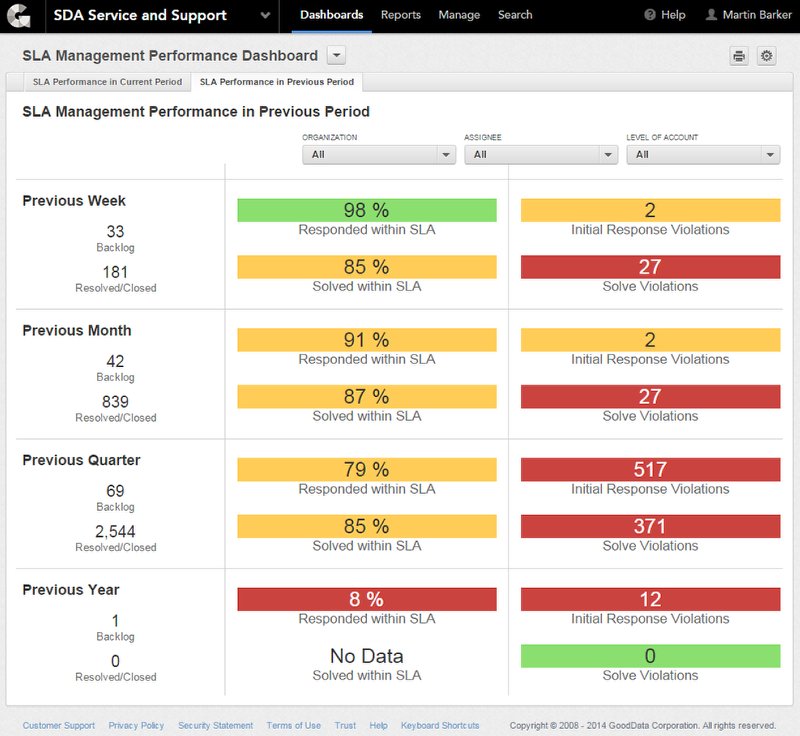
\includegraphics[width=30em]{immagini/sla/slainterface.png}
\caption{Schermata esemplificativa della soluzione ad hoc di interfaccia SLA Manager}
\end{figure}

Questo strumento software sarà già stato utilizzato durante le attività di avviamento e resterà l'interfaccia di riferimenti per il personale dell'Istituto. Verrà rilasciata una versione definitiva e stabile, che la nostra organizzazione si occuperà di mantenere ed evolvere nel tempo, secondo le necessità del business.

%**********************************************************

\section{Sistema informativo del processo di SLA Management}

La base per il sistema informativo del processo di SLA Management è costituita dal software SAP Solution Manager. Le aree cui si dedica sono:

\begin{itemize}
	\item Application Operations;
    \item Business Process Operations;
    \item Data Volume Management;
    \item Change Control Management;
    \item Custom Code Management;
    \item IT Service Management;
    \item Landscape Management;
    \item Process Management;
    \item Project Management;
    \item Test Suite;
    \item Cross Topics;
    \item Focused Solutions.
\end{itemize}

In particolare, esaudisce le richieste riguardo al nuovo processo di SLA Management presentate nel Capitolato Tecnico:

\begin{itemize}
	\item monitoraggio di SLAs, OLAs ed UCs;
    \item consultazione dello stato effettivo del sistema in tempo reale;
    \item documentazione di metriche e KPIs rilevati;
    \item scambio di informazioni tra differenti servizi, dipartimenti ed unità di business;
    \item personalizzazione in base alle specifiche caratteristiche dell'Azienda Ospedaliera;
    \item integrazione con l'ambiente di test per i servizi di sperimentazioni ed innovazioni.
\end{itemize}

Considerando tuttavia la relativa complessità di tale strumento, proponiamo il mantenimento di una soluzione ad hoc per l'interfaccia del sistema informativo denominato SLA Manager. Così facendo, manterremo la qualità di SAP Solution Manager unita alla semplicità di un'interfaccia che interpreti automaticamente le informazioni monitorate. Status, performance, metriche e KPIs dei vari servizi saranno prontamente visibili, aggiornate e soprattutto facilmente comprensibili. Il lato più tecnico sarà comunque disponibile al nuovo dipartimento IT, così da poter lavorare con il massimo dei dati e poter fornire rilevamenti più specifici se necessario.

%**********************************************************

\section{Template documenti}

Di seguito sono riportati dei documenti esemplificativi per:

\begin{itemize}
	\item Service Level Agreements;
    \item Operational Level Agreements;
    \item Underpinning Contracts.
\end{itemize}

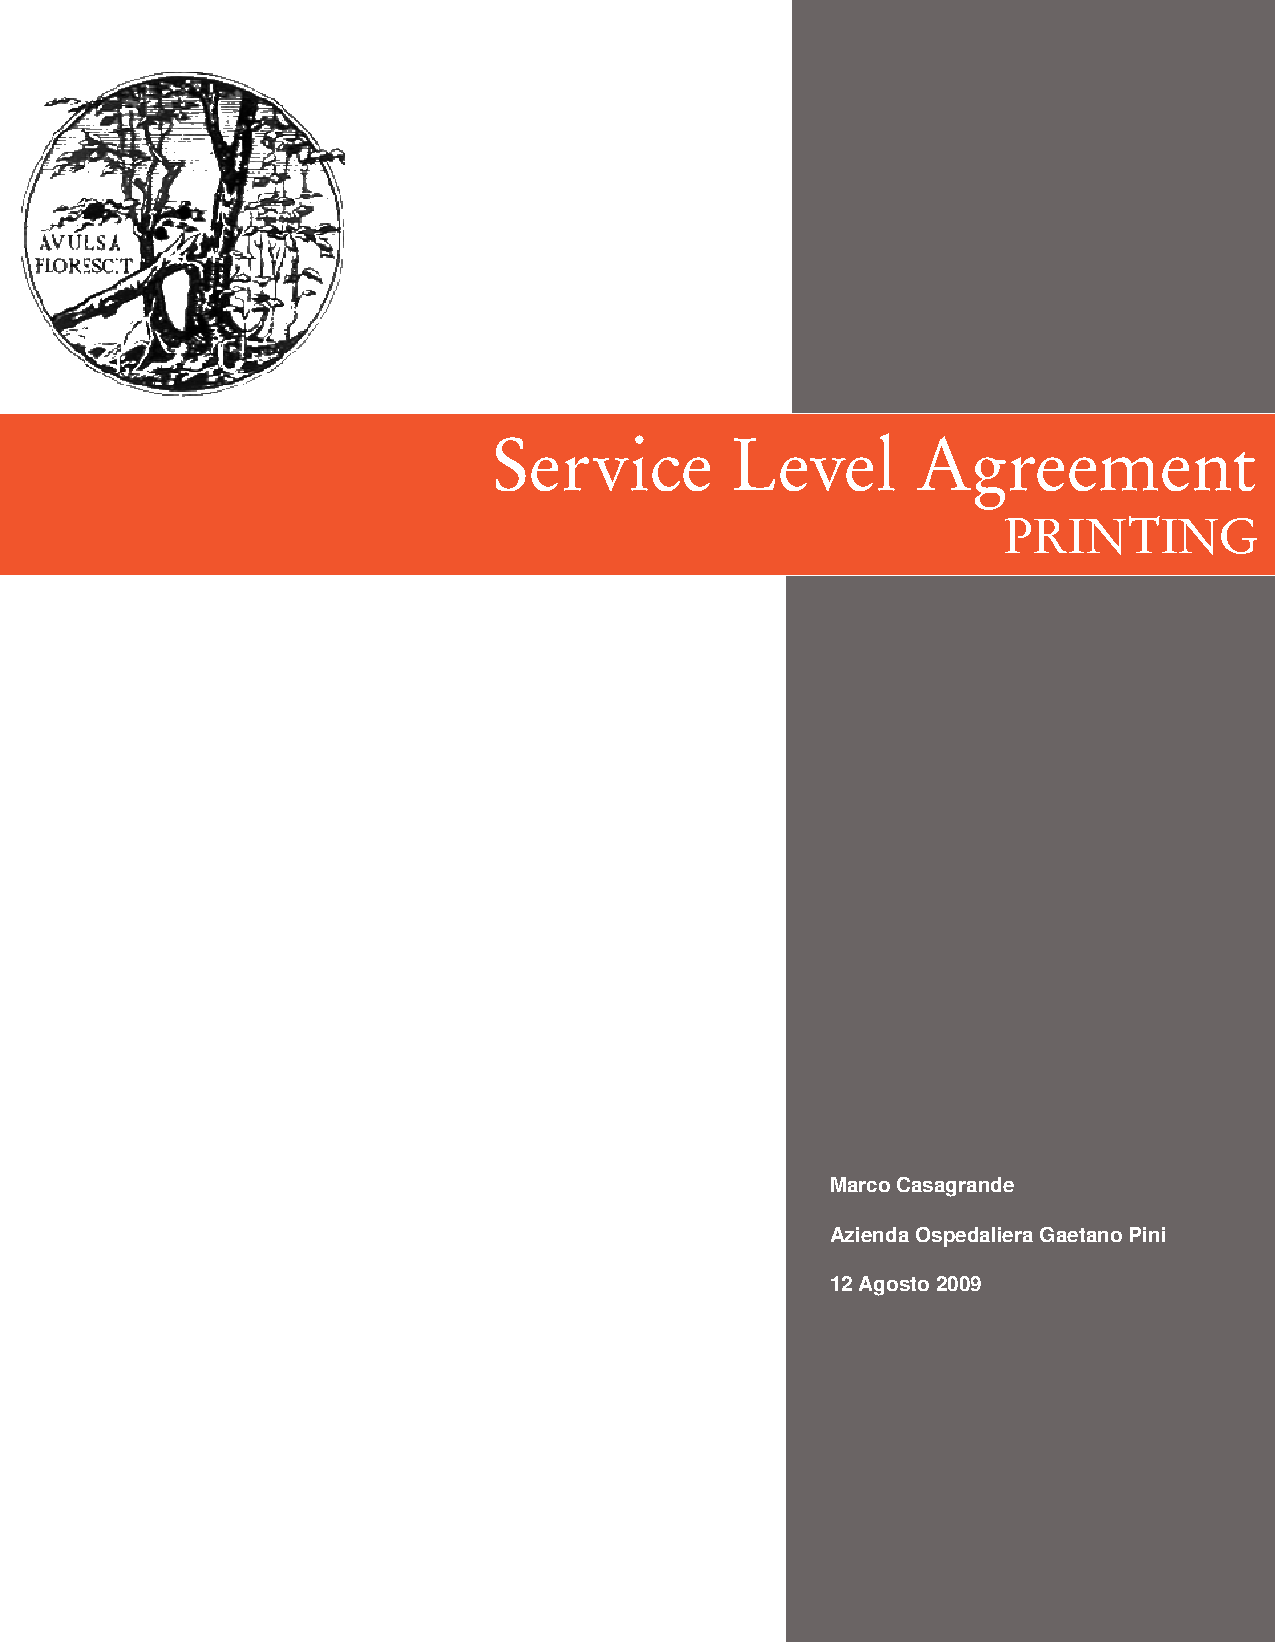
\includepdf[pages=-]{immagini/sla/sla.pdf}


\includepdf[pages=-]{immagini/sla/ola.pdf}


\includepdf[pages=-]{immagini/sla/uc.pdf}
